% Fig. 2.24 / spec Fig A27 -- the empirical rule: the central intervals one,
%   two and three standard deviations either side of the mean, with the
%   probability each of them covers.
% Source: mathstatch2.tex lines 4358-4426.
%
% This file replaces a hand-written SVG (viewBox 760 x 460, not a pdflatex
% product).  Its geometry had already been corrected once and is kept; what is
% fixed here is everything else, the three faults recorded on 2026-08-06:
%   - it was outside the TikZ pipeline, one of the twelve hand-written files
%     of the chapter (the other 49 figures are pdflatex products with their
%     glyphs converted to paths);
%   - its type was 23px against a viewBox 760 wide, i.e. 10.6px at the 350px
%     phone width, under the 12px floor of spec 1.3;
%   - its three shaded blocks were three full rectangles stacked on top of one
%     another inside a clip path, so the levels actually rendered were
%     0.16 / 0.16 / 0.18 and the middle two could not be told apart;
%   - those rectangles were filled in grey (#8f867b) rather than the
%     journalaccent of spec 1.2.
%
% Density: the standard normal, f(x) = 0.3989423 e^{-x^2/2}, drawn over
% |x| <= 3.5.  The x unit IS one standard deviation, so the seven boundaries
% stand at -3, -2, -1, 0, 1, 2, 3 by construction and the mismatch of ERRATA
% C2-21 (manuscript boundaries implying sigma = 1.15 against a curve whose
% sigma is 1.224745) cannot arise.  Curve heights at the boundaries:
%   f(1) = 0.2419707   f(2) = 0.0539910   f(3) = 0.0044318   f(3.5) = 0.0008727
% and the peak f(0) = 0.3989423.  At y = 5cm these stand 1.2099, 0.2700,
% 0.0222 and 1.9947 cm high.
%
% Probabilities, per ERRATA C2-18 and C2-19: 2*Phi(k) - 1 at k = 1, 2, 3 is
% 0.6826894921, 0.9544997361 and 0.9973002039, so to four places
% 0.6827 / 0.9545 / 0.9973 and as percentages 68.27% / 95.45% / 99.73%.  The
% manuscript truncates instead of rounding (68.26 / 95.44 / 99.74 at lines
% 4401, 4407, 4413; 0.6826 / 0.9544 / 0.9974 at lines 4340-4342) and must not
% be followed back.  The figure carries the percentages, as the manuscript
% figure does and as the caption and alt text of P222 both state.
%
% Deviations from CH2_FIGURE_SPECS.md:
%
% 1. Spec 1.6 has a boundary dashed line drop from its point on the curve to
%    the x axis and forbids it to run out above the curve.  That rule is for a
%    figure whose boundaries only cut the area; here each boundary also has to
%    carry an interval arrow drawn clear of the peak, so the six dashed lines
%    rise from the axis, cross the curve and stop 0.10cm above their own arrow
%    row.  This is the manuscript's own arrangement (lines 4373-4413) and the
%    one the reviewed content of this figure has.
%
% 2. Spec 1.3 asks for vertical staggering when neighbouring labels stand
%    closer than 0.6cm.  Here they cannot be brought that far apart on one
%    row: mu-3sigma is 29.32pt = 1.0335cm wide, so a 0.6cm gap needs 1.63cm
%    per standard deviation, i.e. an axis 11.7cm long against the 9.0cm cap of
%    the same section.  The seven labels are therefore staggered, the even
%    multiples (mu-2sigma, mu, mu+2sigma) on the upper row and the odd ones on
%    the lower.  Within a row the labels stand 2 standard deviations = 2.30cm
%    apart, so the gaps are 1.354cm on the lower row and 1.677cm on the upper;
%    between rows the boxes clear each other by 0.116cm horizontally and
%    0.185cm vertically.
%
% 3. Spec 1.2 caps fill opacity at 0.12 to 0.18 but names 0.18 / 0.13 / 0.08
%    for nested shading, which is what this figure needs and uses.  The three
%    levels are laid down as five disjoint paths -- the central block [-1,1],
%    then a ring drawn as its two halves [-2,-1] and [1,2], then a ring as
%    [-3,-2] and [2,3] -- so no point of the picture is covered twice and the
%    rendered levels are the three declared ones, not sums of them.
%
% 4. Spec 1.2 puts fill opacity on journalaccent; the old file used
%    journalmuted grey.  Fixed here.
%
% Size and type.  Native 257.083 x 132.208 pt (drawing range 8.93cm wide,
% inside the 9.0cm cap of spec 1.3).  A mark of S pt shows at
% S x 0.99626 x <display width> / 257.083 px, so for a topic-figure--wide in
% body text, which .topic-figure--wide img sizes at min(100%, 620px), i.e.
% 350px in the 350px article column of a 390px phone,
%     display width      350px (390px phone)   620px (desktop)
%     10pt text          13.56px               24.03px
% Every mark in the picture is at \normalsize: the axis labels, the three
% percentages and the axis name are all 10pt and none of them has a subscript,
% so 13.75px is the smallest type in the figure, not merely the largest.
% \DeclareMathSizes{10}{10}{9}{8} is kept for uniformity with the other files
% of the chapter even though no script size occurs here.
\documentclass[tikz,border=2pt]{standalone}
\usepackage{amsmath}
\usepackage{amssymb}
\usepackage{xcolor}
\usetikzlibrary{arrows.meta}
\DeclareMathSizes{10}{10}{9}{8}

\definecolor{journalink}{HTML}{1F1C18}
\definecolor{journalmuted}{HTML}{8A7F72}
\definecolor{journalaccent}{HTML}{9C2D2D}

% standard normal density, argument in standard deviations
\newcommand{\normaldensity}[1]{0.3989423*exp(-(#1)*(#1)/2)}

\begin{document}
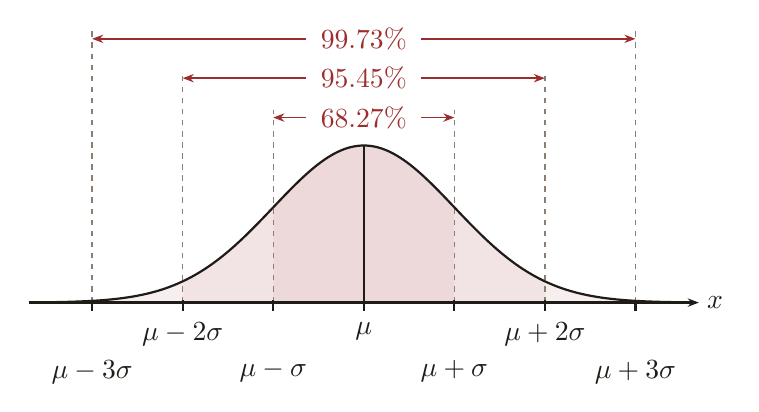
\begin{tikzpicture}[
  x=1.15cm,
  y=5cm,
  every node/.style={font=\normalsize, journalink},
  axis/.style={journalink, line width=0.8pt, -{Stealth[length=4pt]}},
  tick/.style={journalink, line width=0.8pt},
  curve/.style={journalink, line width=0.8pt},
  guide/.style={journalmuted, line width=0.5pt, dash pattern=on 2pt off 2pt},
  meanline/.style={journalink, line width=0.5pt},
  span/.style={journalaccent, line width=0.6pt, -{Stealth[length=4pt]}},
  inner/.style={journalaccent, fill opacity=0.18},
  middle/.style={journalaccent, fill opacity=0.13},
  outer/.style={journalaccent, fill opacity=0.08}
]

  % ---- the three levels of shading, five disjoint paths ----------------
  % Each path follows spec 1.6: from the foot of the left boundary along the
  % x axis to the foot of the right boundary, up to the curve, back along the
  % curve, cycle.  The two rings are drawn as their two halves so that no
  % path ever lies over another one.
  \fill[inner]
    (-1,0) -- (1,0) -- (1,0.2419707)
    -- plot[domain=1:-1, samples=200, smooth] (\x,{\normaldensity{\x}})
    -- cycle;
  \fill[middle]
    (1,0) -- (2,0) -- (2,0.0539910)
    -- plot[domain=2:1, samples=200, smooth] (\x,{\normaldensity{\x}})
    -- cycle;
  \fill[middle]
    (-2,0) -- (-1,0) -- (-1,0.2419707)
    -- plot[domain=-1:-2, samples=200, smooth] (\x,{\normaldensity{\x}})
    -- cycle;
  \fill[outer]
    (2,0) -- (3,0) -- (3,0.0044318)
    -- plot[domain=3:2, samples=200, smooth] (\x,{\normaldensity{\x}})
    -- cycle;
  \fill[outer]
    (-3,0) -- (-2,0) -- (-2,0.0539910)
    -- plot[domain=-2:-3, samples=200, smooth] (\x,{\normaldensity{\x}})
    -- cycle;

  % ---- the seven boundaries --------------------------------------------
  % The six dashed ones rise from the axis, cross the curve and stop 0.10cm
  % above their own arrow row (2.35 / 2.85 / 3.35 cm).  The one at mu is
  % solid and stops at the peak, so that the centre of the distribution is
  % told from the six by line type, not by colour.
  \draw[guide] (-1,0) -- ([yshift=2.45cm]-1,0);
  \draw[guide] ( 1,0) -- ([yshift=2.45cm] 1,0);
  \draw[guide] (-2,0) -- ([yshift=2.95cm]-2,0);
  \draw[guide] ( 2,0) -- ([yshift=2.95cm] 2,0);
  \draw[guide] (-3,0) -- ([yshift=3.45cm]-3,0);
  \draw[guide] ( 3,0) -- ([yshift=3.45cm] 3,0);
  \draw[meanline] (0,0) -- (0,0.3989423);

  % ---- density curve ---------------------------------------------------
  \draw[curve] plot[domain=-3.5:3.5, samples=300, smooth]
    (\x,{\normaldensity{\x}});

  % ---- x axis, ticks and staggered labels ------------------------------
  \draw[axis] (-3.7,0) -- (3.7,0);
  \node[anchor=west, inner sep=2.8pt] at (3.7,0) {$x$};

  \foreach \p in {-3,-2,-1,0,1,2,3}
    \draw[tick] ([yshift=0.035cm]\p,0) -- ([yshift=-0.106cm]\p,0);

  % upper row: the even multiples
  \node[anchor=north, inner sep=0pt] at ([yshift=-0.25cm]-2,0)
    {$\mu-2\sigma$};
  \node[anchor=north, inner sep=0pt] at ([yshift=-0.25cm]0,0) {$\mu$};
  \node[anchor=north, inner sep=0pt] at ([yshift=-0.25cm]2,0)
    {$\mu+2\sigma$};
  % lower row: the odd ones
  \node[anchor=north, inner sep=0pt] at ([yshift=-0.73cm]-3,0)
    {$\mu-3\sigma$};
  \node[anchor=north, inner sep=0pt] at ([yshift=-0.73cm]-1,0)
    {$\mu-\sigma$};
  \node[anchor=north, inner sep=0pt] at ([yshift=-0.73cm]1,0)
    {$\mu+\sigma$};
  \node[anchor=north, inner sep=0pt] at ([yshift=-0.73cm]3,0)
    {$\mu+3\sigma$};

  % ---- the three intervals, innermost lowest ---------------------------
  % Rows at 2.35 / 2.85 / 3.35 cm.  The peak stands 1.9947cm high, so the
  % lowest label box clears it by 0.213cm and the rows clear each other by
  % 0.216cm, both above the 0.18cm of spec 1.3.  A percentage is
  % 31.11pt = 1.0966cm wide, i.e. 0.4768 standard deviations either side of
  % the centre; the arrow tails stand a further 0.18cm out, at 0.6333.
  \node[journalaccent, inner sep=0pt] at ([yshift=2.35cm]0,0) {$68.27\%$};
  \draw[span] ([yshift=2.35cm] 0.6333,0) -- ([yshift=2.35cm] 1,0);
  \draw[span] ([yshift=2.35cm]-0.6333,0) -- ([yshift=2.35cm]-1,0);

  \node[journalaccent, inner sep=0pt] at ([yshift=2.85cm]0,0) {$95.45\%$};
  \draw[span] ([yshift=2.85cm] 0.6333,0) -- ([yshift=2.85cm] 2,0);
  \draw[span] ([yshift=2.85cm]-0.6333,0) -- ([yshift=2.85cm]-2,0);

  \node[journalaccent, inner sep=0pt] at ([yshift=3.35cm]0,0) {$99.73\%$};
  \draw[span] ([yshift=3.35cm] 0.6333,0) -- ([yshift=3.35cm] 3,0);
  \draw[span] ([yshift=3.35cm]-0.6333,0) -- ([yshift=3.35cm]-3,0);

\end{tikzpicture}
\end{document}
